\section{Короткі теоретичні відомості}
\subsection{Розв’язання диференціальних рівнянь}

Диференціальні рівняння~--- розділ математики, який вивчає теорію та способи розв'язування рівнянь, що містять шукану функцію та її похідні різних порядків одного аргументу (звичайні диференціальні) чи кількох аргументів (диференціальні рівняння в частинних похідних). Диференціальні рівняння широко використовуються на практиці, зокрема для опису перехідних процесів.

Теорія диференціальних рівнянь~--- розділ математики, що займається вивченням диференціальних рівнянь і пов'язаних з ними задач. Їх результати застосовуються в багатьох природничих науках, особливо широко~--- у фізиці.

Простіше кажучи, диференціальне рівняння~--- це рівняння, в якому невідомою величиною є деяка функція. При цьому, в самому рівнянні бере участь не тільки невідома функція, але й різні її похідні. Диференціальним рівнянням описується зв'язок між невідомою функцією та її похідними. Такі зв'язки віднаходяться в різних областях знань: у механіці, фізиці, хімії, біології, економіці та ін.

Розрізняють звичайні диференціальні рівняння і диференціальні рівняння в частинних похідних. Більш складними є інтегро-диференціальні рівняння.

Звичайні диференціальні рівняння~--- це рівняння виду:
    \begin{equation}\label{eq:simple_difur}
        F(t,x,x',x'',x^{(n)}) =0,
    \end{equation}

де $x=x(t)$~--- невідома функція (можливо, вектор-функція; в такому випадку часто говорять про систему диференціальних рівнянь), що залежить від змінної часу $t$, штрих означає диференціювання по $t$. Число $n$ називається порядком диференціального рівняння.

У випадку, коли додаткові умови задаються при одному значенні незалежної змінної, має місце задача Коші (задача з початковими умовами). Якщо умови задаються для двох або більше значень незалежної змінної, то задача стає крайовою. У задачі Коші додаткові умови називаються початковими, а у крайовій задачі~--- граничними. При розв’язанні цих задач використовуються різні методи і алгоритми.

Задачу Коші можна сформулювати таким чином.

Нехай дано диференціальне рівняння першого порядку:
\begin{equation}\label{eq:difur_1st}
  \frac{dy}{dx} = f(x,y)
\end{equation}

Потрібно знайти функцію на відрізку від $ {x=a} $ до $ {x=b} $, що задовольняє як рівняння~\eqref{eq:difur_1st}, 
так і початкову умову $y(a) = y_0$ (при цьому завжди припускається, що існує єдиний розв’язок на всьому відрізку).

Задача, що полягає в розв’язанні звичайного диференціального рівняння при додаткових умовах, які поставлені при декількох значеннях незалежної змінної, називається крайовою.
Постановки і методи розв’язання рівнянь більш високих порядків аналогічні.

\subsection{Методи розв’язання задачі Коші}

Основою чисельних методів розв’язання диференціальних рівнянь слугує розкладання функції y в ряд Тейлора в околі початкової точки:
\begin{equation}\label{eq:tailor}
  y(x_0+h) = y(x_0)+hy'(x_0)+
  \frac{1}{2}h^2y''(x_0)+\cdots
\end{equation}

де $h$~--- відстань (крок) між початковою точкою $x_0$ і точкою $x_1=x_0 + h$, в якій відшукується розв’язок.

В різних методах враховується різна кількість членів розкладання ( в
багатокрокових методах в поєднанні з інтерполяційними формулами),
що визначає точність обчислень. При використанні цих методів на ЕОМ
слід розрізняти похибки округлення через обмеженість кількості значущих
цифр в ЕОМ; похибка зрізання (обмеження)~--- методична похибка,
що пов’язана з апроксимацією розв’язків скінченними рядами,
замість нескінченних, наприклад, а. 

Внаслідок цих причин виникають два види похибок:
\begin{enumerate}
  \item локальна~--- сума похибок, що вносяться в обчислювальний
    процес на конкретному кроці;
  \item глобальна (сумарна)~--- різниця між точним і обчисленим
    значеннями, яка включає так звану похибку розповсюдження
    внаслідок накопичення помилок на попередніх етапах обчислення.
\end{enumerate}

Порядок методу дорівнює $p$, якщо існує таке позитивне число $c$, що
\begin{equation}\label{eq:delta}
  \Delta \le ch^{p+1},
\end{equation}

де ${\Delta}$~--- локальна похибка на кроці, ${h}$~--- крок дискретизації.

Число $с$ не залежить від номера кроку і його величини, а визначається
похідними і довжиною інтервалу. При апроксимації розв’язання рядами
Тейлора воно зв’язане зі степенем членів ряду, які відкидаються.

Методи розв’язання задачі Коші поділяють на однокрокові
та багатокрокові.

В однокрокових методах для знаходження наступної точки на
кривій $y=f(x)$ потрібна інформація лише про один попередній крок
(методи Ейлера і Рунге-Кутта).

В багатокрокових методах (прогнозу і корекції) для знаходження 
наступної точки на кривій $y=f(x)$ потрібна інформація більш ніж 
про одну з попередніх точок. Щоб отримати достатньо точне 
чисельне значення часто використовується ітераційна процедура 
(наприклад, в методах Мілна-Адамса, Башфорта, Хеммінга).

\subsubsection{Метод Ейлера}\label{sss:E1}

Найбільш простим однокроковим методом, який потребує мінімальних затрат обчислювальних ресурсів, але дає змогу обчислювати результат із порівняно низькою точністю, є метод Ейлера.

В цьому методі для оцінки наступної точки на кривій y=f(x) використовується лише один лінійний член в формулі Тейлора, 
\begin{equation}
  y(x_0+h)=y(x_0)+hy'(x_0),
\end{equation}

    де $y'(x)$ визначається з початкового рівняння.

    Цей процес можна розповсюдити на наступні кроки:
\begin{equation}
  y_{n+1}=y_{n}+hf(x_n,y_n).
\end{equation}

    Метод Ейлера є методом першого порядку ($p=1$):
\begin{equation}\label{eq:error}
  \Delta \le ch^{2},
\end{equation}
    
    де $c=(M_1+M_0M_2)/2$, $M_0$, $M_1$, $M_2$~--- визначаються як:
\begin{equation}
  \begin{split}
    M_0 &\ge |f(x,y)|,\\
    M_1 &\ge \left|\frac{df(x,y)}{dx}\right|,\\
    M_2 &\ge \left|\frac{df(x,y)}{dy}\right|,
  \end{split}
\end{equation}
 
для всіх $x \in [a,b]$ і $y=y(x)$.

Метод Ейлера, крім значної похибки зрізання часто буває нестійким 
(малі локальні помилки призводять до значного збільшення глобальної).

Цей метод можна вдосконалити різними способами.

\subsubsection{Виправлений метод Ейлера}\label{sss:E2}

Ітераційні формула для цього методу має вигляд:
\begin{equation}\label{eq:E2}
    y_{n+1}=y_n+\frac{h}{2}(f(x_n,y_n)+f(x_n+h,y_n+hf(x_n,y_n)))
\end{equation}

Графічне зображення методу подане на рисунку \ref{img:E2}.

%\begin{figure}[h]
%    \center{\input{images/e2-utf8.tpx}}
%    \caption{Виправлений метод Ейлера}\label{img:E2}
%\end{figure}
\input{images/e2-utf8.tpx}

\subsubsection{Модифікований метод Ейлера}\label{sss:E3}

Ітераційні формула для цього методу має вигляд:
\begin{equation}\label{eq:E3}
    y_{n+1}=y_n+\frac{h}{2}(f(x_n,y_n)+f(x_n+h,y_n+hf(x_n,y_n)))
\end{equation}

Графічне зображення методу подане на рисунку \ref{img:E3}.

%\begin{figure}[h]
%    \center{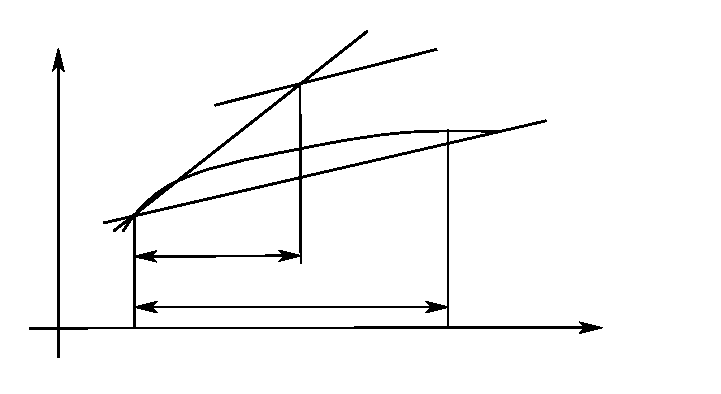
\includegraphics{e3}}
%    \caption{Модифікований метод Ейлера}\label{img:E3}
%\end{figure}
\input{images/e3-utf8.tpx}

Принцип, на якому побудований модифікований метод Ейлера,
можна пояснити, користуючись рядом Тейлора і зберігаючи в ньому
член з $h^2$. Апроксимація другої похідної $y''(x_0)$ здійснюється кінцевою різницею:
\begin{equation}\label{eq:E3_riz}
  y''(x_0)=\frac{\Delta y}{\Delta x}=\frac{y(x_0+h)-y'(x_0)}{h}
\end{equation}

Аналогічно обчисленню другої похідної в кінцево-різницевому
вигляді можна обчислити більш високі похідні: значення
$n$-ї за значеннями попередньої $(n-1)$-ї.  

\subsubsection{Метод Рунге-Кутта}\label{sss:E4}

Метод Рунге-Кутта дає набір формул для обчислення координат
внутрішніх точок, які потрібні для реалізації цієї ідеї.
Оскільки існує ряд способів знаходження цих точок, то метод
Рунге-Кутта об’єднує цілий клас методів для розв’язання
диференціальних рівнянь першого порядку.

Найбільш розповсюджений класичний метод четвертого порядку 
точності:

\begin{equation}\label{eq:E4}
  y_{n+1}=y_n+\frac{k_0+2k_1+2k_2+k_3}{6},
\end{equation}

де
\begin{equation}\label{eq:E4_k}
  \begin{split}
    k_0 &= hf(x_n,y_n);\\
    k_1 &= hf(x_n+\frac{h}{2},y_n+\frac{k_0}{2});\\
    k_2 &= hf(x_n+\frac{h}{2},y_n+\frac{k_1}{2});\\
    k_3 &= hf(x_n+h,y_n+k_2).
  \end{split}
\end{equation}

Метод Ейлера і його модифікації ще називають методами
Рунге-Кутта першого і другого порядку. Метод Рунге-Кутта має
значно більш високу точність, що дозволяє збільшити крок
розв’язання. Його максимальну величину визначає припустима
похибка. Такий вибір часто здійснюється автоматично і
включається як складова частина в алгоритм, побудований за
методом Рунга-Кутта.

\subsection{Розв'язання диференціальних рівнянь вищих порядків}

Будь-яку з формул Рунге-Кутта можна використовувати для
розв’язання диференціальних рівнянь вищих порядків і систем
диференціальних рівнянь. Рівняння порядку $n$ можна звести до
$n$ диференціальних рівнянь першого порядку.

Як приклад розглянемо розв'язання звичайного диференціального
рівняння другого порядку:

\begin{equation}\label{eq:difur_2st}
  \frac{d^2y}{dx^2} = g\left({x,y,\frac{dy}{dx}}\right).
\end{equation}

Введемо заміну $z=\dfrac{dy}{dx}$, 
тоді $\dfrac{dz}{dx}=\dfrac{d^2y}{dx^2}$,
а рівняння \eqref{eq:difur_2st} прийме вигляд системи:

\begin{equation}\label{eq:system_2_difurs}
    \left\{
    \begin{aligned}
      \dfrac{dz}{dx}&= g(x,y,z);\\
      \dfrac{dy}{dx}&= f(x,y,z),
    \end{aligned}
    \right.
\end{equation}

де $f(x,y,z)=z$.

Задача Коші в цьому випадку містить дві початкових умови:

\begin{equation}\label{eq:poch_um}
    \left\{
    \begin{aligned}
      y(x_0)&= y_0;\\
      z(x_0)&=y'(x_0)=z_0.
    \end{aligned}
    \right.
\end{equation}

Розв'язавши систему рівнянь \eqref{eq:system_2_difurs} отримаємо
розв'язок диференціального рівняння \eqref{eq:difur_2st}, що
задовольнятиме задані початкові умови \eqref{eq:poch_um}.

\subsection{Обчислення похибок}\label{ss:errors}

В розділі \ref{sss:E1} було зазначено, що помилка зрізання при
використанні методів Рунге-Кутта $n$-го порядку визначається за
формулою \eqref{eq:error}. Обчислення верхніх границь для
коефіцієнта с являє собою складну задачу, пов’язану з необхідністю
оцінки ряду додаткових параметрів. Існує декілька способів для
оперативного обчислення $с$. Найбільшого поширення набув
екстраполяційний метод Річардсона (ще його називають методом Рунге),
коли послідовно знаходять значення $y_n$ з кроком $h$ і з кроком
$\dfrac{h}{2}$, а після цього прирівнюють отримані величини та
визначають $c$ з рівняння:

\begin{equation}\label{eq:tochnoe}
  y = y_{n}^{(h)}+ch^{p+1} =
  y_{n}^{\left(\frac{h}{2}\right)}+
  c\left(\dfrac{h}{2}\right)^{p+1}
\end{equation}

де $y$~--- точне значення на даному кроці.

Отримаємо оціночне співвідношення:

\begin{equation}\label{eq:c}
  c=\frac{y_{n}^{(h)}-y_{n}^{\left(\frac{h}{2}\right)}}
        {h^{p+1}-\left(\dfrac{h}{2}\right)^{p+1}}
\end{equation}